%! TEX root = ../000-main.tex
\chapter[Introduction]{Introduction to unsupervised learning}

\section{Supervised and unsupervised learning}

\paragraph{References:} Section 14.1 of \cite{hastie_elements_2009}

\subsection{Supervised learning}

\begin{definition}{Supervised learning}{supervised-learning}\index{supervised learning}
	(prediction problem)

	It is a learning problem where the aim is to predict the value of a
	\iemph{response variable} $y$ given a set of \iemph{explanatory variables} $X$
	(features).

	\begin{description}
		\item[Regression] Predict a continuous value.
		\item[Classification] Predict the class of an observation. (qualitative variable)
	\end{description}

	\tcblower

	The main interest is the conditional distribution $P(y \mid X)$.

\end{definition}

\subsection{Unsupervised learning}

\begin{definition}{Unsupervised learning}{unsupervised-learning}\index{unsupervised learning}
	Aims to learn relationships and structure in the observed data.

	We don't have a response variable $y$.

	\tcblower

	The main interest is the conditional distribution $P(X)$.

\end{definition}

\begin{example}{Problems in unsupervised learning}{}
	\tcbline
	\begin{description}
		\item[Density estimation] Learn the distribution of the data.
		\item[Clustering] Find groups of similar observations.
		\item[Dimensionality reduction] Find a low-dimensional representation of the data.
		\item[Extraction of latent variables] Proposing generative probabilistic models for $X$
			depending on low-dimensional unobservable random variables $F$ (Factor analysis).
	\end{description}
\end{example}

\pagebreak
\section{Density estimation}

\paragraph{References:} Section 6.6 of \cite{hastie_elements_2009}, Chapter 6 in \cite{wasserman_all_2006}

Let's assume that $\mathbf{X} = X$ is a one-dimensional continuous random variable.

\begin{definition}{Density function}{}
	A function $f$ is a density function of $X$ if $\forall a < b \in \mathds{R}$:
	\begin{equation*}
		P(a < X \leq b) = \int_a^b f(x) \, dx
	\end{equation*}
\end{definition}

Let $dx \geq 0$ be a small length. Let $0 \leq u \leq dx,\; v = dx - u$. Then:
\begin{align*}
	f(x) \approx \frac{P(X \in [x, x + dx])}{dx} \approx \frac{P(X \in [ x - u, x + v])}{dx} \\
	f(x) \approx \frac{\text{probability}}{\text{length}}
\end{align*}
Given $x_1, \ldots, x_n$ i.i.d.%
\index{iid}%
\footnote{\iemph{independent and identically distributed}}
samples from $X$, we want to estimate the density function $f$
at $x$ in a non-parametric way.

\begin{definition}{non-parametric}{non-parametric}\index{non-parametric}
	A method is non-parametric if it does not make any assumptions about the
	distribution of the data.
\end{definition}

\subsection{The histogram}
It is a very simple non-parametric density estimator.

\begin{definition}{histogram}{histogram}\index{histogram}
	A histogram is a non-parametric density estimator that consists of a sequence of
	rectangles, each of which has a height proportional to the density at the center of
	the rectangle.
	\tcblower
	Formally:
	\begin{equation*}
		\widehat{f}_H(x) = \sum_{j=1}^m \frac{p_j}{b_j - b_{j-1}} I_{B_j}(x)
	\end{equation*}
\end{definition}

The appearance of the histogram strongly depends on the choice of the bin width $b$,
as we can see in \cref{fig:histogram_bins}.

\begin{note}
	The performance of the histogram as an estimator depends on the bin width $b$:
	\begin{itemize}
		\item If $b$ is too large \textrightarrow high bias and low variance.
		\item If $b$ is too large \textrightarrow low bias and high variance.
	\end{itemize}
\end{note}

\begin{figure}[H]
	\begin{tikzpicture}
		\begin{axis}[
				xlabel=LSTAT,
				ylabel=Density,
				width=0.3\textwidth,
				ymax=0.08
			]
			\addplot+[mark=none,hist={density,bins=5}] table[y index=12,col sep=comma] {data/boston.csv};
		\end{axis}
	\end{tikzpicture}
	\begin{tikzpicture}
		\begin{axis}[
				xlabel=LSTAT,
				ylabel=Density,
				width=0.3\textwidth,
				ymax=0.08
			]
			\addplot+[mark=none,hist={density,bins=15}] table[y index=12,col sep=comma] {data/boston.csv};
		\end{axis}
	\end{tikzpicture}
	\begin{tikzpicture}
		\begin{axis}[
				xlabel=LSTAT,
				ylabel=Density,
				width=0.3\textwidth,
				ymax=0.08
			]
			\addplot+[mark=none,hist={density,bins=50}] table[y index=12,col sep=comma] {data/boston.csv};
		\end{axis}
	\end{tikzpicture}
	\caption{Histograms of \texttt{LSTAT} from Boston Housing data with different $b$}%
	\label{fig:histogram_bins}
\end{figure}

\begin{definition}{Bias}{bias}
	The bias of an estimator is the difference between the expected value of the
	estimator and the true value of the parameter being estimated.
\end{definition}

\begin{definition}{Variance}{variance}
	The variance of an estimator is the expected value of the squared deviation of the
	estimator from its expected value.
\end{definition}

\subsection{Kernel density estimator}

Let's now introduce the \iemph{kernel density estimator}, a non-parametric
density estimator that outperforms the histogram.

It is smooth, continuous and respects the data distribution characteristics.

\begin{figure}[H]
	\begin{tikzpicture}
		\begin{axis}[
				xlabel=LSTAT,
				ylabel=Density,
				ymax=0.08
			]
			\addplot+[mark=none,hist={density,bins=50}] table[y index=12,col sep=comma] {data/boston.csv};
			\addplot [thick] gnuplot [raw gnuplot] {
					set key autotitle columnhead;
					set datafile separator ",";
					plot 'data/boston.csv' u 13:(1./500.) smooth kdensity
				};
		\end{axis}
	\end{tikzpicture}
	\caption{Histogram and kernel density estimator of \texttt{LSTAT} from Boston Housing data}%
\end{figure}

The kernel density estimator provides two improvements over the histogram:
\begin{itemize}
	\item Localization
	\item Smoothing
\end{itemize}

\subsubsection{Localization (Moving histogram)}
\begin{prop}{The histogram estimates better at the center of the bin}{}
	It can be proven that the histogram estimates better the density at the center of the
	bin than at the edges.
	\tcblower
	Let $x$ be the point at which we want to estimate the density.

	We force $x$ to be in the center of one of the histogram intervals:
	\begin{equation*}
		B_x = \left[ x - \frac{b}{2}, x + \frac{b}{2} \right] = [ x - h, x + h ]
	\end{equation*}

	The estimator will be:
	\begin{align*}
		\widehat{f}_U(x) & = \frac{1}{n}\sum_{i=1}^n \frac{1}{b} I_{[x - b/2, x + b/2]}(x_i)                  \\
		                 & = \frac{1}{n}\sum_{i=1}^n \frac{1}{2h} I_{[-1, 1]}\left( \frac{x_i - x}{h} \right)
	\end{align*}

	If we want to estimate at a different point $x'$, we move the interval again.
\end{prop}

\subsubsection{Smoothing (Moving average)}
\begin{prop}{$\widehat{f}_U(x)$ is not smooth}{}
	Since it is discontinuous and piecewise constant due to the use of the indicator
	function $I_{[-1,1]}$.
	\tcblower
	If we want to smooth the estimator, we can use a kernel function $K$ (that is twice derivable) instead
	of the indicator function resulting in a density estimator that inherits the
	smoothness properties:
	\begin{equation}
		\widehat{f}_K(x) = \frac{1}{n}\sum_{i=1}^n K\left( \frac{x_i - x}{h} \right)
		\tag{kernel density estimator}
	\end{equation}
	This is called the \iemph{kernel density estimator}.

	$K$ is the \iemph{kernel function}, which is a continuous density function, unimodal
	and symmetric around $0$.

	$h$ is known as the \iemph{smoothing parameter} or \iemph{bandwidth} and is a
	\iemph{hyperparameter} of the estimator.
\end{prop}

The kernel density estimator spreads the weight $\frac{1}{n}$ of each
observation in its neighborhood in a continuous way.

\begin{definition}{Unimodal}{unimodal}
	A function $f$ is unimodal if it has only one maximum.
\end{definition}

\begin{definition}{Symmetric}{symmetric}
	A function $f$ is symmetric around a point $x_0$ if $f(x) = f(x_0 - (x - x_0)) \quad \forall x$.
\end{definition}

\subsubsection{Bandwidth selection}
\begin{marker}{}
	This is the key point of the kernel density estimator:

	\begin{description}
		\item[large bandwidth] very stable from sample to sample (low variance) but with a large bias
		\item[small bandwidth] very sensitive to the sample (high variance) but with a small bias
	\end{description}
\end{marker}

There is extensive literature on the topic of bandwidth selection, but we will
focus only on maximum likelihood cross-validation.

\begin{definition}{Maximum likelihood cross-validation}{mlcv}
	(for bandwidth selection)

	For a given bandwidth $h$, the likelihood of observation $x_i$ is evaluated
	using the density estimator computed from the other elements in the sample:
	\begin{equation*}
		\hat{f}_{h,(-i)}(x_i) = \frac{1}{(n-1)h}\sum_{j \neq i}^n K\left( \frac{x_i - x_j}{h} \right)
	\end{equation*}
	The sample likelihood is the product of the likelihood of each observation:
	\begin{equation*}
		\mathcal{L}_{CV}(h) = \prod_{i=1}^n \hat{f}_{h,(-i)}(x_i)
	\end{equation*}
	We look for the value $h_{LCV}$ that maximizes the previous expression.
	\tcblower
	This method is simple and can be used for choosing the tuning parameters of any density estimator.
\end{definition}



\subsection{Multivariate density estimation}\index{multivariate density estimation}

Let $\boldsymbol{x_1}, \dots, \boldsymbol{x_n}$ be $n$ i.i.d. observations
from the $p$-dimensional variable $\boldsymbol{X}$ having density
function $f(\boldsymbol x),\,\boldsymbol x \in \mathbb{R}^p$.

For a given $\boldsymbol x \in \mathbb{R}^p$, we want to estimate $f(\boldsymbol x)$.

Natural generalization of the 1-dimensional density estimator:
\begin{equation*}
	\widehat{f}_K(\boldsymbol{x}) = \frac{1}{n}\sum_{i=1}^n
	\frac{1}{|H|}K_p\left(
	H^{-1}\left(\boldsymbol{x} - \boldsymbol{x_i}\right)
	\right)
\end{equation*}
where:
\begin{align*}
	H   & = p \times p \text{ non-singular \iemph{bandwidth matrix}}                             \\
	K_p & : \mathbb{R}^p \to \mathbb{R} \text{ \iemph{kernel function} in } p \text{-dimensions}
\end{align*}

\begin{definition}{Non-singular matrix}{non-singular}
	A matrix $A$ is non-singular if $A^{-1}$ exists.
\end{definition}

Usually, $K_p$ is a $p$-dimensional density function centered at $\boldsymbol{0} \in \mathbb{R}^p$.
Then, $\hat{f}_K(\boldsymbol{x})$ is a mixture of densities, each of them centered at one of
the observations $\boldsymbol{x_i} \in \mathbb{R}^p$.

\begin{figure}[H]
	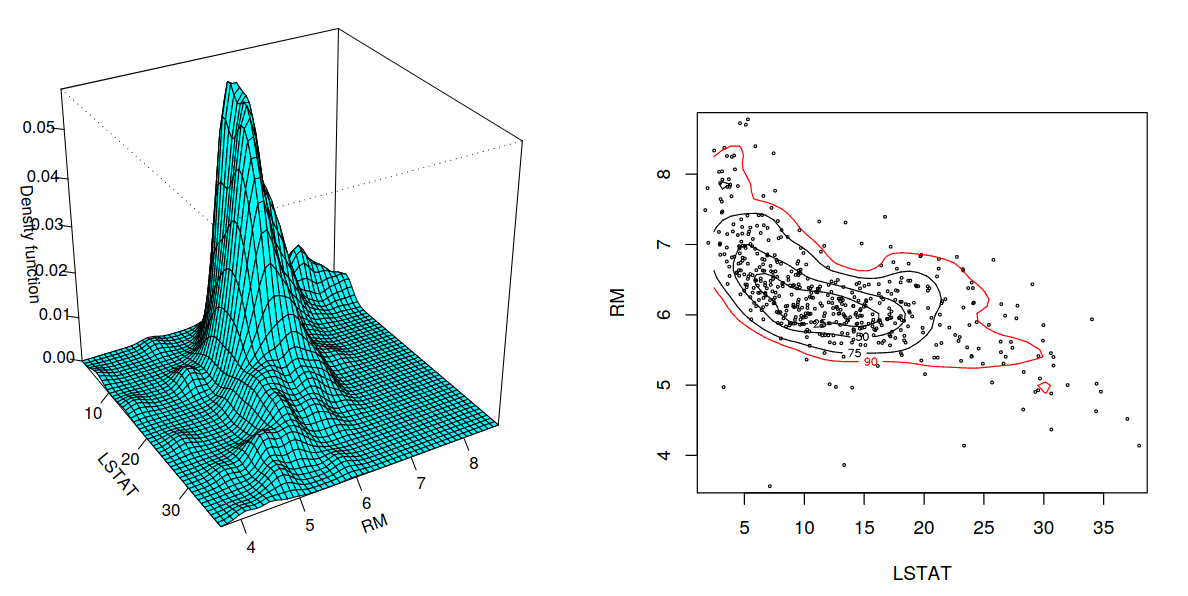
\includegraphics{figures/multivariate-kernel-density}
	\caption{Kernel estimator for the joint density function of variables
		\texttt{LSTAT} and \texttt{RM} in the \texttt{Boston} dataset.}
\end{figure}

\subsection{The curse of dimensionality}%
\label{sec:curse-of-dimensionality}%
\index{curse of dimensionality}
A general problem in multivariate non-parametric estimation, and in
particular in non-parametric density estimation, is the phenomenon
known as the curse of dimensionality:
\begin{quote}
	In high dimensional spaces the neighborhood of any point contains
	virtually no observational data.
\end{quote}

\begin{marker}
	Non-parametric estimation of the density function (or any other
	function) is extremely difficult when the data dimension $p$ is large
	(in practice $p \geq 4$).
\end{marker}

\subsection{Software}
Density estimation in R:
\begin{itemize}
	\item Functions \texttt{hist}, \texttt{density}. Bandwidth choice: \texttt{bw.nrd}, \texttt{bw.ucv},
	      \texttt{bw.bcv}, \texttt{bw.SJ}
	\item Package \texttt{KernSmooth}, functions \texttt{bkde} (for density estimation) and
	      \texttt{dpik} (for bandwidth choice). See also \texttt{dpih}. \cite{wand_kernel_1994}
	\item Package \texttt{sm}, functions \texttt{sm.density} (for density estimation) and
	      h.select (for bandwidth choice). \cite{bowman_applied_1997}
	\item Package \texttt{ks}, function \texttt{kde} for density estimation and several
	      functions for bandwidth choice. Well suited for multivariate density
	      estimation for 1- to 6-dimensional data. \cite{chacon_multivariate_2018}
\end{itemize}

\pagebreak
\section{Mixture models}
\paragraph{References:} \cite[Sections 6.8 and 12.7]{hastie_elements_2009}, \cite[Section 13.1.3]{fan_statistical_2020}, \cite[Chapter 10]{lange_numerical_1999}

\subsection{Mixture of two distributions}

The assumption that the true density function $f(\boldsymbol{x})$ follows
a \iemph{mixture model} is useful for density estimation when $p$ is \emph{large}.

\begin{definition}{Mixture Model}{mixture-model}
	\begin{equation*}
		f(\boldsymbol{x}) = \sum_{j=1}^k \alpha_j f_j(\boldsymbol{x}),\quad \alpha_j \geq 0,\quad \sum_{j=1}^k \alpha_j = 1
	\end{equation*}

	For a certain $k \geq 1$ and $p$-dimensional density functions $f_1, \dots, f_k$,
	which are assumed to be much simpler than $f(\boldsymbol{x})$.
\end{definition}

\begin{definition}{Parametric Mixture Model}{}\index{parametric mixture model}
	\begin{equation*}
		f(\boldsymbol{x}) = \sum_{j=1}^k \alpha_j f_j(\boldsymbol{x}\mid\boldsymbol{\theta}_j)
	\end{equation*}
\end{definition}

\begin{example}{Gaussian Mixture Model}{}\index{gaussian mixture model}
	\begin{equation*}
		f(\boldsymbol{x}) = \sum_{j=1}^k \alpha_j \phi(\boldsymbol{x}\mid \mu_j, \Sigma_j)
	\end{equation*}
	Where $\phi(\boldsymbol{x}\mid \mu, \Sigma)$ is the multivariate Gaussian density function
	with mean vector $\mu$ and covariance matrix $\Sigma$.
\end{example}

\begin{definition}{Model-based clustering}{}\index{model-based clustering}
	Clustering based on a parametric mixture model.
\end{definition}

\subsubsection{Mixture of two distributions (example)}

Let $(X,\,Y)$ be a bivariate random variable:
\begin{align*}
	Y               & \sim \text{Bernoulli}(p),                                               \\
	( X \mid Y = 0) & \sim f(x;\,\theta_0),                                                   \\
	( X \mid Y = 1) & \sim f(x;\,\theta_1)                                                    \\[0.5em]
	F_X(x)          & = Pr(X \leq x)                                                          \\
	                & = Pr(X \leq x \mid Y = 0) Pr(Y = 0) + Pr(X \leq x \mid Y = 1) Pr(Y = 1) \\
	                & = p F(x;\,\theta_0) + (1-p) F(x;\,\theta_1)                             \\
	                & \Downarrow                                                              \\
	f_X(x)          & = F'_X(x) = p f(x;\,\theta_0) + (1-p) f(x;\,\theta_1)
\end{align*}
$f_X(x)$ is the mixture of $f(x;\,\theta_0)$ and $f(x;\,\theta_1)$.

We observe $n$ independent observations $(x_1,\,y_1),\dots,(x_n,\,y_n)$ from $(X,\,Y)$:
\begin{alignat*}{2}
	\boldsymbol{x} & = (x_1,\,\dots,\,x_n)       & \boldsymbol{y} & = (y_1,\,\dots,\,y_n) \\
	\boldsymbol{X} & = (X_1,\,\dots,\,X_n) \quad & \boldsymbol{Y} & = (Y_1,\,\dots,\,Y_n)
\end{alignat*}

\paragraph{Likelihood function from the complete data}
\begin{align*}
	L(p,\theta_0,\theta_1;\,\boldsymbol{x},\boldsymbol{y})
	 & = \prod_{i=1}^n f(x_i \mid Y_i = y_i) Pr(Y_i = y_i)                                       \\
	 & = \prod_{i=1}^n f(x_i;\, \theta_1)^{y_i} f(x_i;\, \theta_0)^{1-y_i} p^{y_i} (1-p)^{1-y_i}
\end{align*}

The log-likelihood function is:
\begin{align*}
	\span \ell(p,\theta_0,\theta_1;\,\boldsymbol{x},\boldsymbol{y})
	= \log L(p,\theta_0,\theta_1;\,\boldsymbol{x},\boldsymbol{y})       \\
	 & = \sum_{i=1}^n \left( y_i \log p + (1 - y_i) \log(1 - p) \right)
	+ \sum_{i:y_i=1} \log f(x_i;\,\theta_1)
	+ \sum_{i:y_i=0} \log f(x_i;\,\theta_0)                             \\
	 & = \sum_{i=1}^n y_i \log \frac{p}{1-p} + n \log (1 - p)
	+ \sum_{i:y_i=1} \log f(x_i;\,\theta_1)
	+ \sum_{i:y_i=0} \log f(x_i;\,\theta_0)
\end{align*}

\subparagraph{Maximum likelihood estimation}
\begin{equation*}
	\hat{p}^{ML} = \sum_{i=1}^n \frac{y_i}{n}
\end{equation*}
For $j = 0,1$; $\hat{\theta}_j^{ML}$ is the maximum likelihood estimator of $\theta$ from the subsample
of $x_i$ corresponding to $y_i = j$.

\begin{note}
	It could be the case that $\hat{p}^{ML}$ can be calculated using a closed-form solution
	(e.g. Mixture of two Gaussians). But even if it is not the case, the optimization
	problem is easier than direct maximization with respect to $p,\theta_0,\theta_1$.
\end{note}

\paragraph{Likelihood function from the incomplete data}

If we only observe data from $X$ the likelihood function is:
\begin{align*}
	L(p,\theta_0,\theta_1;\,\boldsymbol x)    & = \prod_{i=1}^n f_X(x_i)                                                         \\
	                                          & = \prod_{i=1}^n \left( p f(x_i;\,\theta_1) + (1-p) f(x_i;\,\theta_0) \right)     \\[1em]
	\ell(p,\theta_0,\theta_1;\,\boldsymbol x) & = \sum_{i=1}^n \log \left( p f(x_i;\,\theta_1) + (1-p) f(x_i;\,\theta_0) \right)
\end{align*}

In this case, the MLE involves ($p,\theta_0,\theta_1$) jointly.
And \emph{very rarely} we can find a closed-form solution for the MLE.

Unfortunately, the standard situation is that the data is incomplete
(the indicator variables $Y_1,\dots,Y_n$ are not observed).

\begin{question}{Can we have an optimization problem similar to that of the complete data
		$(X,\,Y)$ even if we observe only the incomplete data $X$?}{}
	Yes, we can use the EM algorithm.
\end{question}

\subsection{The EM algorithm}\index{EM algorithm}

Since the complete data log-likelihood $\ell(p,\theta_0,\theta_1;\,\boldsymbol{X},\boldsymbol{Y})$
cannot be computed when only incomplete
data $\boldsymbol{X}$ is observed, we maximize its conditional expectation given
$\boldsymbol{X} = \boldsymbol{x}$ instead:
\begin{align*}
	E \left(\ell(p,\theta_0,\theta_1;\,\boldsymbol{X},\boldsymbol{Y}) \mid \boldsymbol{X}=\boldsymbol{x} \right)
	= & \sum_{i=1}^n E(Y_i \mid \boldsymbol{X}=\boldsymbol{x}) \log \frac{p}{1-p} + n \log (1 - p) \\
	  & + \sum_{i=1}^n E(Y_i \mid \boldsymbol{X}=\boldsymbol{x}) \log f(x_i;\,\theta_1)            \\
	  & + \sum_{i=1}^n (1 - E(Y_i \mid \boldsymbol{X}=\boldsymbol{x})) \log f(x_i;\,\theta_0)
\end{align*}

\subsubsection{The E(xpectation)-step}
$(Y_i \mid \boldsymbol{X}=\boldsymbol{x})$ is a Bernoulli random variable with parameter
$p = P(Y_i = 1 \mid \boldsymbol{X}=\boldsymbol{x})$. Thus, by Bayes' theorem:
\begin{align*}
    E(Y_i \mid \boldsymbol{X}=\boldsymbol{x}) & = P(Y_i = 1 \mid \boldsymbol{X}=\boldsymbol{x})
    \propto f_{\boldsymbol{X}}(\boldsymbol{x} \mid Y_i = 1) P(Y_i = 1) \\
                                              &= \prod_{h=1}^n f_{X_h}(x_h \mid Y_i = 1) P(Y_i = 1)
                                              \propto f_X(x_i \mid Y_i = 1) P(Y_i = 1) = f_X(x_i;\,\theta_1) p
\end{align*}
Analogously: $P(Y_i = 0 \mid \boldsymbol{X}=\boldsymbol{x}) = f_X(x_i;\,\theta_0) (1-p)$.

Using that $P(Y_i = 1 \mid \boldsymbol{X}=\boldsymbol{x}) + P(Y_i = 0 \mid \boldsymbol{X}=\boldsymbol{x}) = 1$,
and assuming that $p, \theta_0, \theta_1$ are known:
\begin{align*}
    P(Y_i = 1 \mid \boldsymbol{X}=\boldsymbol{x}) & = \frac{f_X(x_i;\,\theta_1) p}{f_X(x_i;\,\theta_1) p + f_X(x_i;\,\theta_0) (1-p)} \tag{$\hat{y}_i$}\\
    P(Y_i = 0 \mid \boldsymbol{X}=\boldsymbol{x}) & = \frac{f_X(x_i;\,\theta_0) (1-p)}{f_X(x_i;\,\theta_1) p + f_X(x_i;\,\theta_0) (1-p)}
\end{align*}

Let
\begin{align*}
    \hat{y}_i & = E(Y_i \mid \boldsymbol{X}=\boldsymbol{x}) ) =
    P(Y_i = 1 \mid \boldsymbol{X}=\boldsymbol{x}) \\
              &= \frac{f_X(x_i;\,\theta_1) p}{f_X(x_i;\,\theta_1) p + f_X(x_i;\,\theta_0) (1-p)}
              = \hat{y}_i(p,\theta_0,\theta_1)
\end{align*}

\subsubsection{The M(aximization)-step}
We want to maximize the conditional expectation of the log-likelihood function:
\begin{align*}
    E \left(\ell(p,\theta_0,\theta_1;\,\boldsymbol{X},\boldsymbol{Y}) \mid \boldsymbol{X}=\boldsymbol{x} \right)
    = & \left(
        \sum_{i=1}^n \hat{y}_i \log \frac{p}{1-p} + n \log (1 - p)
        \right) \\
      & + \sum_{i=1}^n \hat{y}_i \log f(x_i;\,\theta_1) + \sum_{i=1}^n (1 - \hat{y}_i) \log f(x_i;\,\theta_0)
\end{align*}

If we consider $\hat{y}_i$ as fixed (ignoring its dependence on $p, \theta_0, \theta_1$), the
previous function is the sum of 3 functions, each depending on a single parameter:
\begin{alignat*}{2}
    \max_{p}&\left( \sum_{i=1}^n \hat{y}_i \log \frac{p}{1-p} + n \log (1 - p) \right) & \quad \rightarrow{} \quad
    \hat{p} & = \frac{\sum_{i=1}^n \hat{y}_i}{n} \\
    \max_{\theta_1}&\sum_{i=1}^n \hat{y}_i \log f(x_i;\,\theta_1) \\
    \max_{\theta_0}&\sum_{i=1}^n \hat{y}_i \log f(x_i;\,\theta_0)
\end{alignat*}

$\hat{\theta}_1$ and $\hat{\theta}_0$ are the weighted maximum likelihood estimates
of $\theta$ with weights $\hat{y}_i$ and $1 - \hat{y}_i$, respectively.

\begin{marker}
    The \emph{EM-algorithm} consists of iterating the E-step and the M-step until convergence.
\end{marker}

\subsection{Software}
\begin{itemize}
	\item Package \texttt{ClusterR}
	      \begin{itemize}
		      \item \texttt{GMM}: fits a Gaussian mixture model to the data using the EM algorithm.
		      \item \texttt{Optimal\_Clusters\_GMM} to determine the optimal number of clusters.
		      \item Also includes other clustering methods such as $k$-means and $k$-medoids.
	      \end{itemize}
	\item Package \texttt{mclust}: model-based clustering, classification and density estimation
        based on finite normal mixture modeling.
	      \begin{itemize}
		      \item \texttt{Mclust}: Model-based clustering based on parameterized finite
                  Gaussian mixture models. Modesl are estimated by EM algorithm. The optimal
                  model is selected by \iemph{BIC} (Bayesian Information Criterion).
	      \end{itemize}
	\item Package \texttt{fpc}, Flexible Procedures for Clustering:
	      \begin{itemize}
		      \item \texttt{mergenormals}: Clustering by merging components of a Gaussian mixture.
		      \item \texttt{cluster.stats}: Computes several cluster validity statistics from a
		            clustering and a dissimilarity matrix.
	      \end{itemize}
\end{itemize}

\pagebreak
\section{Density based clustering}
\paragraph{References:} \cite{ester_density-based_1996}
\subsection{DBSCAN}

Density-Based Spatial Clustering of Applications with Noise (DBSCAN) is
a density-based clustering algorithm that is able to find clusters of
arbitrary shape.

\begin{definition}{Density-based clusters}{}\index{density-based clusters}
	Connected areas of the sample space with high \emph{density of observations}.
\end{definition}

\begin{definition}{Outliers (noise)}{}
	Observed points that are not part of any cluster.
\end{definition}

\subsection{Measuring the density of observations}
Let $\mathcal{D} = \{ \boldsymbol{x}_1, \ldots, \boldsymbol{x}_n \}$ be a set of $n$ observations
in a $p$-dimensional space. For each observation $\boldsymbol{x}_i$, we define the $\varepsilon-$\iemph{neighborhood}
of $\boldsymbol{x}_i$ as the set of points $\boldsymbol{x}_j$ such that:
\begin{equation*}
    N_{\varepsilon}(\boldsymbol{x}_i) = \bigl\{
    \boldsymbol{x}_j \in \mathcal{D} \mid d(\boldsymbol{x}_i,\,\boldsymbol{x}_j) \leq \varepsilon
    \bigr\}
\end{equation*}
where $d(\boldsymbol{x}_i,\,\boldsymbol{x}_j)$ is a distance measure between points in $\mathds{R}^p$.

The \iemph{density of observations} around $\boldsymbol{x}_i$ is estimated by the number
of observations at $N_{\varepsilon}(\boldsymbol{x}_i)$.

Observe that this is proportional to:
\begin{equation*}
    \hat{f}_\varepsilon(\boldsymbol{x}_i) =
    \frac{|N_{\varepsilon}(\boldsymbol{x}_i)| / n}{\text{Volume}(N_{\varepsilon}(\boldsymbol{x}_i))}
    = \frac{|N_{\varepsilon}(\boldsymbol{x}_i)| / n}{\text{Volume}(\varepsilon^p N_{1}(\boldsymbol{0}))}
\end{equation*}
which is the kernel estimator of the probability density function at $\boldsymbol{x}_i$
when using an uniform kernel on $\mathds{R}^p$ and bandwidth of $\varepsilon$.

\subsubsection{Main concepts}
\begin{definition}{Core point}{}\index{core point}
    A point $\boldsymbol{x}_i$ is a \emph{core point} if $|N_{\varepsilon}(\boldsymbol{x}_i)| \geq \text{minPts}$.

    That is, if the estimated density of observations around $\boldsymbol{x}_i$ is over a certain threshold.
\end{definition}

\begin{definition}{Border point}{}\index{border point}
    A point $\boldsymbol{x}_i$ is a \emph{border point} if it is not a core point but it is
    in the $\varepsilon-$neighborhood of a core point.
\end{definition}

\begin{definition}{Noise point (or outlier)}{}\index{noise point}
    A point $\boldsymbol{x}_i$ is a \emph{noise point} if it is not a core point and it is not a border point.
\end{definition}

\begin{definition}{Densly connected}{}\index{densly connected}
    Two points $\boldsymbol{x}_0$ and $\boldsymbol{x}_{m+1}$ are \emph{densly connected} if
    there is a path of \emph{core points} $\boldsymbol{x}_1, \ldots, \boldsymbol{x}_{m}$ such
    that $d(\boldsymbol{x}_i,\,\boldsymbol{x}_{i+1}) \leq \varepsilon$ for all $i = 0, \ldots, m$.

    \tcblower
    Observe that $\boldsymbol{x}_0$ and/or $\boldsymbol{x}_{m+1}$ can be core or border points.
\end{definition}

\begin{definition}{Cluster}{}\index{cluster}
    
    Clusters are subsets of density-connected points (all the points in the cluster are
    density-connected) which are maximal (if a point $\boldsymbol{x}_i$ is density-connected
    with another point $\boldsymbol{x}_j$, then both points are in the same cluster).

    \tcblower

    Only core and border points can be part of a cluster.

    Outliers are not part of any cluster.

    The number of clusters is not known in advance.

    The core points in a DBSCAN cluster are a subset of observed points belonging to the same
    connected component of the level set of the estimated density function:
    \begin{equation*}
        \left\{
            \boldsymbol x \in \mathds{R}^p \mid \hat{f}_\varepsilon(\boldsymbol x) \geq f_0
        \right\}
    \end{equation*}
    where the threshold $f_0$ is: $\frac{\text{minPts}}{n \cdot \varepsilon^p \text{Volume}(N_{1}(\boldsymbol{0}))}$.
    
\end{definition}

\subsubsection{DBSCAN Algorithm}

\begin{marker}
There are two hyperparameters in DBSCAN: $\varepsilon$ and $\text{minPts}$.
\end{marker}

\begin{figure}[H]
    \begin{algorithmic}[1]
    \Procedure{DBSCAN}{$\varepsilon$, minPts}
        \State Mark each point $\boldsymbol{x}_i$ as either core, border or noise
        \State Remove all noise points
        \State $j \gets 0$
        \While{There are still core points}
            \State Select a random core point $\boldsymbol{x}_i$
            \State Define a new cluster $C_j$ with $\boldsymbol{x}_i$
            \State Add to $C_j$ all points density-connected to $\boldsymbol{x}_i$
            \State Add to $C_j$ all border points density-connected to $\boldsymbol{x}_i$
            \State Remove all points in $C_j$ from the set of core points
            \State $j \gets j + 1$
        \EndWhile
    \EndProcedure
\end{algorithmic}
\end{figure}

\begin{figure}[H]
    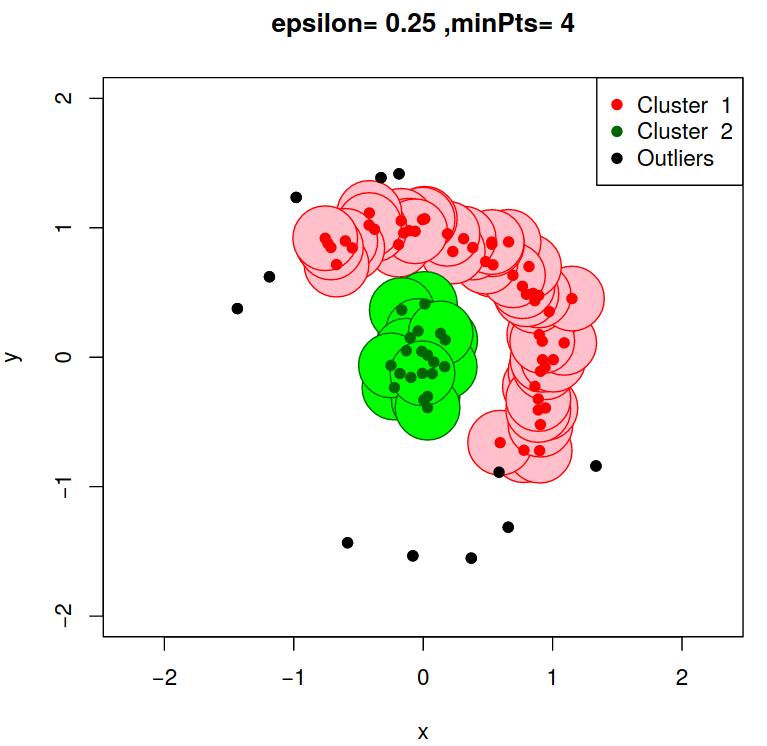
\includegraphics[width=0.6\textwidth]{../figures/dbscan_eps_minpts}
    \caption{Visualization of the DBSCAN algorithm}
\end{figure}

\subsection{Software}

\begin{itemize}
	\item Package \texttt{fpc}, Flexible Procedures for Clustering:
	      \begin{itemize}
		      \item \texttt{dbscan}: Computes DBSCAN density based clustering as introduced
		            in \cite{ester_density-based_1996}.
		      \item \texttt{cluster.stats}: Computes several cluster validity statistics from a
		            clustering and a dissimilarity matrix.
	      \end{itemize}
	\item Package \texttt{dbscan}, function \texttt{dbscan}: Fast reimplementation of the
	      DBSCAN.
\end{itemize}
